
%%%%%%%%%%%%%%%%%%%%%%%%%%%%%%%%%%

\part{Preparing for Wikipedia data analysis}

%%%%%%%%%%%%%%%%%%%%%%%%%%%%%%%%%%

\chapter{Understanding Wikipedia data sources}

\setlength{\epigraphwidth}{.5\textwidth}
\epigraph{``It is a capital mistake to theorize before one has data. Insensibly 
 one begins to twist facts to suit theories, instead of theories to suit facts''.}
 {\textit{A Scandal in Bohemia}, Sir Arthur Conan Doyle, 1892.}

The first step in data analysis is always to find an interesting question or a
set of questions (sometimes expressed as hypotheses) that we want to answer 
or validate. Then, we search out for data to answer these questions or assess 
the validity of our hypotheses.

Once we have found promising data sources, we need to collect these data, load
or store them somewhere, and start the exploratory phase of data analysis (a.k.a.
EDA). In this stage, we compute numerical scores and graphics to describe our data set, in order to
validate its adequacy for the purposes of our study. We must also
pay attention to detect any special traits or anomalies in our data set (missing values, extreme
values, incorrect labeling, etc.) that could undermine the validity of our analysis.

It is very curious to realize how this important stage of data analysis is usually
overlooked in scientific reports. Space limitations in research publications
(journals, tech reports, conference papers, etc.) often force authors to
concentrate on the initial premises, results and discussion, which are the sections
delivering the actual scientific contribution. However, this also makes quite
difficult for other researchers to replicate the results of previous studies
and extend the analysis beyond its initial scope. This is particularly true for
works involving very large data sets, such as many studies featuring Wikipedia.

Over the past 5 years, I have reviewed numerous scientfic works and reports dealing
with Wikipedia data analysis. To my surprise, I still can find recurrent problems
linked to incorrect assumptions about the nature of the process generating the
data and their meaning, issues with data preparation (unfiltered items introducing
noise or that are irrelevant for the purposes of the study), and many other hurdles
that jeopardize the validity of new promising research works.

My aim in this guide is to (hopefully) help you to avoid commiting these common
pitfalls in your own studies or, in case you are also limited by space constraints
in your own reports, to circumvent these obstacles so that you can condunct your
own analyses with confidence. To achieve this, the first step is to learn all
necessary details about Wikipedia data and available information sources that you
can use to retrieve them.

\section{Public data sources}
The first important characteristic of Wikipedia data sources is that many useful
data records are publicly available for download and use. This include information
about Wikipedia content, discussion pages, user pages, editing activity (who, what and
when) administrative tasks (reviewing content, blocking users, deleting or moving
pages), and many, many other details.

The main exception to this general rule is private data about Wikipedia users who
registered in any of the more than 280 different languages available in Wikipedia
(more on this in the next section). This is for a very good reason: it is not my
business or your business to learn about the real name or e-mail address of Wikipedia
users. Privacy must be preserved and Wikimedia Foundation does a splendig job in
this regard. In any case, editors who registered for an account in a Wikipedia
language have a unique nickname that is associated to their account, and that 
is displayed as their public identifier whenever they perform any action in the
wiki. For the purpose of tracking activity of individual contributors, this 
should suffice for most of your studies. As we will see later on, there is no
reliable method to discriminate contributions from anonymous users, though.

At the same time, this also means that Wikipedia offers detailed records about all
activity performed by users, turning Wikipedia into a public space compliant with the design
principles of \textit{social translucence}~\cite{Erickson1999} in digital systems. Of course, that means
that we can virtually track the complete activity history of every single user in
Wikipedia. However, from a research ethics point of view, despite many users are
fully aware that their digital footsteps can be traced in detail, some of them may
not feel very comfortable if they are pinpointed in a study. So as a researchers,
we also have the responsibility of reporting this information with care, and avoid
unnecessary precise details in our results for the sake of respecting some of the
\textit{public privacy} of Wikipedia users (in particular, without obtaining their
explicit consent).

In summary, Wikipedia offers a vast and quite rich data garden for researchers
and practitioners, which is public and made available through some convenient 
channels that we will discover in the next sections. Let's start our walk 
through the Wikipedia data store.

\section{Different languages, different communities}
\label{sec:langs-communities}
Another important aspect of Wikipedia is that a different MediaWiki~\footnote{\url{http://www.mediawiki.org/wiki/MediaWiki/}} 
site is maintained for every different language in Wikipedia. Therefore, editors
who want to contribute to more than one language with a user account must
register for a new account in each new language. Since May 27, 2008, a unified login feature has
been deployed to facilitate users with presence in multiple language to perform
simultaneous login in all of them in a single step~\footnote{\url{http://en.wikipedia.org/wiki/Wikipedia:Unified_login}}.
However, many users find that their nickname in one language has already
been taken by another person in a different language. This is a very common 
scenario for older user accounts.

As a consequence, in general we must stick with the assumption that nicknames
in Wikipedia identify users only within a certain language community, and that they
do not identify users consistently accross different languages, unless we can
prove otherwise reliably.

Besides, having different communities also means that they may follow distinct
policies, guidelines or conventions to organize editorial and maintenace tasks, as
well as interactions among community members. Admittedly, all languages
follow at least the central organizational priciples underpinning the
whole Wikipedia project, such as 
\textit{the five pillars}~\footnote{\url{http://en.wikipedia.org/wiki/Wikipedia:Five_pillars}}.
Nevertheless, customized policies and guidelines can include some variations that alter substantive
characteristics of the activity that generates data and metadata from a
given language. For instance, whereas in many languages administrator privileges 
(\textit{sysop}) are granted permanently (unless revoked for some good reasons), 
administrators in the Norwegian Wikipedia must renew their special status periodically. 
Another example is the habit extended in the Polish Wikipedia of deleting talk 
pages that remain idle for some time, thus inducing us to infer (somewhat 
incorrectly) that their interesting in debates on articles contents is unusually 
low.

\section{Activity vs. requests}
Wikipedia not only offers data about \textit{actions
that change the status of the system} (edits, page moving or deletiong, blocking users,
etc.) but also about \textit{requests that do not alter content or the status of the system}.
A clear example of the latter is page views (requests to Wikipedia servers to display
a wiki page on our web browser). Other examples include searches performed on the site or
clicking on the edit or preview button while changing the content of a wiki page
(but without clicking on the save button, which is the action actually recorded on
the system database).

We can call this data about requests that do not modify the status of the system 
\textit{requests data}, while \textit{activity data} will refer to actions actually
modifying the status of the system. We are not going to cover requests data in this
guide. The main reason is that only some of this data, namely for page views, is
publicly available~\footnote{\url{http://stats.grok.se/}}. However, in case that
you are interested in obtaining a sampling for all possible actions in Wikipedia
traffic data (both requests and activity data) you must contact the 
\textit{Wikipedia Research Committee}~\footnote{\url{http://meta.wikimedia.org/wiki/Research:Committee}} 
directly to ask for a data stream containing that sample. This data stream will be,
in all cases, conveniently anonymized to elid all private information about users
performing requests to the system. The stream usually includes a sample of the
whole data stream, frequently following a 1:100 ratio.

If you are interested in learning more about the type of analyses that
we can conduct with this data, I recommend you to grab a good cup of your favourite
stimulating beverage and take a look at the doctoral thesis written by my colleague
Antonio J. Reinoso~\cite{reinoso2011} about Wikipedia traffic~\footnote{By no means
I meant with this that reading Antonio's thesis is a boring activity. He did quite
a remarkable work and it is written in clear style. All the same, reading any PhD.
dissertation is always a daunting task, as you are often exposed to many more
intrincate details than you usually need. May the wiki Force be with
you!}.

\section{Activity in Wikipedia}
One of the first questions that newcomers to Wikipedia data analysis usually ask
themselves is: what kind of data is available? What is recorded? What can I
access? In this section, I briefly present a summary of the editorial and maintenance
process in Wikipedia, to understand what kind of activity data is generated and
stored in the system database.

Wikipedia is ``\textit{the free encyclopedia that anyone can edit}''. Therefore, the
first aspect we must take into account is that any person in the world can change
any page in any Wikipedia language. Moreover, you do not need to register for
a user account to edit in Wikipedia. \textit{Anonymous editors} are persons who
edit Wikipedia without a user account. In that case, the system only stores an
identifier, the so-called IP address, of the source (computer system) from 
which the incoming edit request was created. One might think that this is 
enough to differeantiate anonymous editors from each other, but this is not true. 

The explanation is related to some technical details about a low-level, essential 
communication protocol in the Internet known as Internet Protocol (IP). To take
a simple example, consider a shared network connection at home, where all devices
must first connect to a single router to access the Internet. Let's assume
that three different persons are connected at the same time to your router,
all of them editing Wikipedia pages without a user account. In that case, all three
outgoing connections will share, from the perspective of the Wikipedia system, 
the same IP address. The reason is that the router sends outgoing connections identified
by its own IP address, instead of using the IP address of the individual devices
(which are private, just valid inside your own home network). In larger corporate
or campus networks, the situation can be the same, and tens or hundreds of devices
can send outgoing traffic sharing the same IP address of devices filtering content
or routing communication traffic. The result is that we cannot distinguish different
anonymous editors from each other.

However, if the editor has logged in before starting any activity that changes everything.
In that case, any action performed by this person will be recorded in the database,
associated with a \textit{unique numerical identifier} as well as a \textit{username},
identifying that user account. In this case, users can do many more things than
just editing, for example creating new pages (article, talk pages, user pages, etc), or
editing semi-protected pages (pages protected from being edited by anonymous contributors,
due to frequent episodes of vandalism). Registered users with special privileges can
also perform administrative actions such as renaming, moving or deleting pages. As we
will see in Section~\ref{sec:dump-files}, editing and administrative actions are
logged in different dump files. 

A timestamp of the form \texttt{YYYY-MM-DD HH:MM:SS} is also 
recorded in any database entry, to keep track of the exact time at which any 
action was performed on the system. Remember that different Wikipedia languages
are hosted in different MediaWiki instances, each one with its own database, independent
from each other. Likewise, recall that it is not straightforward to follow the
activity of the same registered user in different languages, as we explained
in Section~\ref{sec:langs-communities}. 

From the point of view of the wiki, an edit on any page creates a new version of
that page, with the updated content. If a new page was created, then a new entry
in the database is created to assign a new \textit{unique numerical identifier} to
that page. Deleted pages are removed from the public are of the system database and
all information associated to them is moved to a special private area, not available
in the public dumps. Nevertheless, the dump file for administrative actions do track
these actions.

\subsection{Useful definitions}
\label{subsec:methodology-definitions}

At this point, we can develop some definitions to help us develop more precise
descriptions in the rest of this companion guide:

\paragraph{Namespace}: Each of the logical areas in which the content of any wiki
based on MediaWiki is classified. The database stores, for each wiki page, a numerical
identifier indicating which namespace it belongs to. The \texttt{main} namespace, with
numerical code 0, corresponds to Wikipedia articles. Table~\ref{tab:wkp-namespaces} 
exhibits a complete list of frequent namespaces that can find in any Wikipedia
language. For languages other than English, some or all textual names for namespaces
are translated into that language, whereas the numerical codes should remain the same.

\begin{center}
   \begin{longtable}{|l|l|}
   \caption{List of most relevant namespaces in the Wikipedia 
    database (for each language edition, though we present the English version names)}
   \label{tab:wkp-namespaces}\\
   \hline
    {\bfseries Namespace ID} & {\bfseries Namespace}\\
   \hline
    -2 & Media\\
    \hline
    -1 & Special\\
    \hline
    {\bfseries 0} & {\bfseries Main (blank name)}\\
    \hline
    {\bfseries 1} & {\bfseries Talk} \\
    \hline
    {\bfseries 2} & {\bfseries User}\\
    \hline
    {\bfseries 3} & {\bfseries User\_talk}\\
    \hline
    4 & Wikipedia\\
    \hline
    5 & Wikipedia\_talk\\
    \hline
    6 & Image\\
    \hline
    7 & Image\_talk\\
    \hline
    8 & MediaWiki\\
    \hline
    9 & MediaWiki\_talk\\
    \hline
    10 & Template\\
    \hline
    11 & Template\_talk\\
    \hline
    12 & Help\\
    \hline
    13 & Help\_talk\\
    \hline
    14 & Category\\
    \hline
    15 & Category\_talk\\
    \hline
    
%    \end{supertabular}
%   \end{centering}
   \end{longtable}
  \end{center}

\paragraph{Page}: Any wiki page, disregarding the namespace in which it is stored in the
system database, whose information can be edited. This includes
encyclopedic articles, user pages, discussion pages associated with each article 
(\texttt{talk\_pages}), etc. Any page can be \textbf{\textit{uniquely}} identified by their
corresponding \textit{numerical page identifier} in the database.

\paragraph{Article}: A page in the Main namespace, that contains an encyclopedic article.
  
% \paragraph{Featured Article (FA)}: An article that has deserved to be nominated as one of the
% top quality articles produced in a certain language edition of Wikipedia. The nomination takes
% place after an exhaustive reviewing process performed by all interested members of the community,
% upon an open call issued by the corresponding responsible in that language version.
% Candidate articles are proposed by community members to enter this reviewing process. The result
% of a voting process, reflecting the opinions of all reviewers involved, determines whether the article
% is promoted to this new status or not. The promotion is not permanent, that is, as soon as community members
% detect that the quality of the article has lowered, they can suggest the article as a candidate for a
% new reviewing process. In case that the FA does not pass this review, it can be demoted again
% to its original non-FA status.

\paragraph{Redirect}: A special type of article, with no content at all. Their purpose
is to link to alternative encyclopedic entries for a certain term. 

% \paragraph{Stub}: An article considered so short as to be considered as a useful
% encyclopedic article. Stubs are usually new articles recently opened, providing a seed
% upon which to create a longer, more complete encyclopedic entry. They are usually marked
% as such using special \textit{templates}, customized in each language edition (sometimes, even
% for distinct categories in each language version). There is no official policy regarding
% the minimum length an article must attain to avoid being considered a stub.

\paragraph{Talk page}: Wiki pages storing discussion about encyclopedic articles. 
Each talk page is presented next to its corresponding
article in the MediaWiki interface. However, newly created articles does not automatically come
with a talk page, so it may or may not exist (until an editor decides to create it). They are
stored under the \texttt{talk\_page} namespace, with the exception of talk pages associated
to \textit{user pages} (see below), which are stored under the \texttt{user\_talk\_page} namespace.

\paragraph{User page}: Wiki pages presenting information of a \textit{logged author} (see below) in 
a certain language edition (see below). They are stored under the special \texttt{user\_page}
namespace in MediaWiki.

\paragraph{Revision}: Any individual modification on a wiki page in a certain
language edition of Wikipedia, that is registered in the database as such and identified
by a \textit{unique} numeric ID.

\paragraph{Editor/author}: An individual who performed at least one revision in that language
edition under a user account. For privacy reasons, access to the database
table containing the full list of registered users in that language, along with sensible information
like real names or email accounts is not accessible. Editors are identified by a numeric identifier 
in the database, associated to every revision attributed to her. This identifier is different
for registered and anonymous editors.

\paragraph{Registered/logged editor}: Any editor who created a new user account in a 
certain language edition of Wikipedia. Logged editors can be \textbf{\textit{uniquely}} identified by
either their numeric user identifier (\texttt{rev\_user} field) or their username (\texttt{rev\_user\_text}
field) in the \texttt{revision} table of the corresponding database. Therefore, authors
must log in the system before performing revisions, to let the database register
their identity.

\paragraph{Anonymous editor}: Any editor who performs revisions under anonymous identity,
without a user account. Anonymous authors are identified in the database by a common user identifier $\mbox{\texttt{rev\_user}}=0$
and the IP address from which the author contacted the system, which is stored in the
\texttt{rev\_user\_text} field, both corresponding to the \texttt{revision} table in the
database.

\paragraph{Privileged author}: Any logged author who received certain special privileges within
the system, which are stored in the \texttt{user\_groups} table of the database. Many new roles
have been created in Wikipedia to grant special privileges to certain users. Readers can refer
to the Wikipedia page on this subject to find additional information about available levels
and their associated attributions~\footnote{\url{http://en.wikipedia.org/wiki/Wikipedia:User_access_levels}}.

\paragraph{Bot}: Software programs that performs revisions on a Wikipedia language 
in an automated way. Many bots can be uniquely identified due to their special
privileged status \texttt{'bot'} associated with their unique \texttt{rev\_user}, 
recorded in the \texttt{user\_groups} table in the database.

\section{Web scraping}
Now we turn to describe available sources to retrieve Wikipedia activity
data. The first, and probably most obvious one, is to obtain these data from the
information displayed on our browser when we request any Wikipedia page. Some
people could think that retrieving information about Wikipedia articles using
this procedure, known as \textit{web scraping}~\footnote{\url{http://en.wikipedia.org/wiki/Web_scraping}}
is a good option.

I certainly discourage you to follow this path, unless you have very good and
clear reasons supporting that choice. The main argument against this approach is that, if
you try to visit too many pages at a very fast pace to retrieve their content, high
chances are that you get banned by automated control mechanisms in the server
side infrastructure, on the premise of creating an excessive traffic load. 
Moreover, you have other better alternatives providing more information without
the downside of overloading the Wikipedia server infrastructure with too
many requests.

\section{MediaWiki API}
A very useful data retrieval channel for real-time requests lovers is the
MediaWiki API~\footnote{\url{http://www.mediawiki.org/wiki/API:Main_page}}, available
for most (if not all) of the Wikipedia languages. Like many other data retrieval
APIs, it offers a structured syntax to query the Wikipedia system for the
data we are looking for. Queries take the form of HTTP GET requests accepting
various parameters to refine the target and restrictions of our petitions to the 
system.

A big advantage of using the MediaWiki API is that it also ships a \texttt{format}
parameter that let consumers control the format in which the answer is represented.
Available return formats include the most important data representation standards, like
JSON, WDDX, XML, YAML or PHP native serializaton. This is also a good
way to query the MediaWiki database to obtain answers for precise questions or
data subsets that match certain conditions~\footnote{\url{https://www.mediawiki.org/wiki/API:Query}}.
I am not convering available data fields in the server database yet, since
they will be described in section~\ref{sec:dump-files}.

On the other side, we must keep in mind that we should not overuse this
data retrieval channel, specially since some of the queries can be expensive for
Wikipedia servers to resolve in terms of system resources. Admins reserve the right
to ban any user that may abuse this service~\footnote{\url{https://www.mediawiki.org/wiki/API:Etiquette}}.
In summary, this is a flexible and convenient way to send concrete questions to
the system when we know in advance that the answers should not return very large
data sets. It can also be very helpful for software applications that need to query
the Wikipedia system in (almost) real-time. However,
if you are interested in retrieving the complete activity history of the
whole English Wikipedia in this fashion, arm yourself with a high dosis of 
patience or (much better) try one of the other available alternatives.

\section{The toolserver}
The Wikimedia toolserver~\footnote{\url{http://toolserver.org}} is a cluster of
servers operated by Wikimedia Deutschland, with assistance from the Wikimedia 
Foundation, Inc. and supported by Wikimedia UK, Wikimedia Switzerland, 
Wikimedia Austria and Wikimedia Sweden. Its aim is to maintain replicas of databases from
all Wikimedia's project, in order to test new software, provide added-value services
and statistics based on these data, and host research activities. For example,
some of the new statistics about Wikipedia articles are computed by software
services running on this toolserver~\footnote{\url{http://toolserver.org/~tparis/articleinfo/index.php}}.

In order to get access to this infrastructure, interested researchers must contact
the toolserver responsibles to obtain a user account and shell access
\footnote{\url{https://wiki.toolserver.org/view/Account_approval_process}}. 
Before you ask, yes, the servers run on GNU/Linux, so you must have some minimal background about
perfoming connections to remote systems on SSH and basic shell usage. The database
engine to store this replicas is MySQL (the same database used for all Wikimedia 
projects up to know).

The infrastructure is quite powerful, though the usual common sense and etiquette rules
apply here, as well, regarding the use of shared computational resources.

\section{Wikipedia dump files}
\label{sec:dump-files}
The best way to retrieve large portions or the whole set of activity data 
from any Wikipedia language is using the \textit{database dump files}. These
dump files contain precise records about allº editorial and maintenace actions 
performed in any Wikipedia language. Some dump files also contain additional
metadata about content (links to pages outside Wikipedia, link to other pages
in the same Wikipedia language) or editors (for example, users with special
privileges). Depending on the purpose of your study, sometimes you can use
dump files that only contain metadata, which are smaller and let you speed up
the data loading process. However, if you are interested in any aspect about
the content of wiki pages, you must use the whole dumps with the text of all
revisions for whole set of pages in that language.

Dump files for all Wikimedia projects (not only for any Wikipedia language)
are publicly available and they can be retrieved from the Wikimedia 
Downloads center~\footnote{\url{http://dumps.wikimedia.org/}}.
Lately, these centralized repository has also been replicated on some mirrors 
offered by several institutions around the world. They share storage space and 
bandwith \textit{pro bono} to help balancing the load.

These dump files usually have two possible formats for data representation:

\begin{itemize}
 \item \textit{XML files}: XML is the preferred format for large dump files, such
as those storing information about revisions in wiki pages, or administrative and
maintentance actions. XML presents a neutral format to
export this information and recover it locally to another wiki system (for example,
to build a replica of Wikipedia in a given language) or any other storage system.

 \item \textit{SQL files}: SQL files are usually published for small or medium
size dump files, like external or internal links in wiki pages, the list of
redirects, or the list of special users and their associated privileges. 
\end{itemize}

Since these dump files can consume a lot of storage capacity in the servers, it
is a common practice to publish compressed version of these files, using different
algorithms according to the compression rate required to reduce the size of the
files. On one hand, very large dump files like the ones
contanining all revisions recorded in large Wikipedia languages (German, French,
etc.) are compressed in \textit{7-zip} or \textit{bzip2} format. On the other hand, smaller dump
files are compress in \textit{gzip} format, since it can be decompressed at a faster rate 
and we not need the same high compression ratio as in larger dumps.

In the case of the English Wikipedia, the single dump file that was formerly produced
containing all wiki text and metadata for all revisions has
been conveniently split into multiple pieces, slices or \textit{chunks}. Each of 
these chunks contain information about all revisions performed in a range of wiki pages.
The limits of the range (in the form of the unique numerical identifiers assigned
to every page) are indicated in the file name. Other large dumps, like those
containing the abstracts of articles or those including only metadata about
revisions in the wiki (without the wikitext for each version) are also split in
a similar fashion.

An important advantage of retrieving information from these dump files is that
researchers have complete flexibility as for the type and format of the information
they want to obtain. As we will see in the next chapter, this also means that
researchers can search for information about useful metadata present in the wiki
text that was not originally included in the fields of the database. An example
of this could be searching for special tags that mark quality content in
Wikipedia, templates for assessing the status of articles (verifiability, disputed
neutrality) or tracking the evolution of links and references inserted in an
article over time.

Of course, whenever something is too good to be true there must be some hidden
caveat. In this case, the downside is that one needs to use any software already
available to import this information from the dump files, or write their own
code to accomplish this (something that, unfortunately, is not within the reach of many people).
In the next chapter, we will review some existing tools that can help you in this
endeavour. In the next subsection, we will describe in detail the content of some of the most
popular dump files.

Finally, an important remark about the dump files is that every new file 
includes again all data already stored in prior versions,
plus the new changes performed in the system since the last dump process, and
excluding all information and metadata pertaining pages that have been deleted
in that interval. In other words, we must understand these dump files as
\textit{snapshots} of the status of a Wikipedia language (or any other wiki of
a Wikimedia project) at the time in which the dump process was triggered. Now and
then, new people subscribing to the mailing list devoted to discuss the back up process,
status and features of the dump files~\footnote{\url{https://lists.wikimedia.org/mailman/listinfo/xmldatadumps-l}}
asks about the existence of this kind of incremental dump feature. In case that
we only had to deal with new changes, this could certainly be implemented without
too much effort. However, the additional complication introduced by page
deletions makes this way trickier to implement, and less useful (otherwise, the
dump may show information about pages that do not exist in the wiki any more...,
well, unless they are restored again in the future... funny enough, right?).

\subsection{Types of dump files}
\label{subsec:type-dump-files}
If you visit the Wikimedia Downloads center, and click on \textit{database backup dumps}
you will arrive at a page listing the progress of the process to generate all
dump files for every Wikimedia wiki. Clicking on the link with the name of the
project will lead you to the page summarizing all available dump files for it,
along with the links to download them. The project code is easy to 
interpret. Any link of the form \textit{XXwiki}, where XX is a 2-letter (sometimes
3-letter) ISO code representing the language, identifies the Wikipedia in that
language. Therefore, \textit{eswiki} links to the dump files of Wikipedia in
Spanish, \textit{frwiki} to the dumps of the French Wikipedia, and so on.

As an example the filename \textit{frwiki-20120601-pages-meta-history.xml.7z} tells
us that the dump file belongs to the ensemble for the French Wikipedia, the
date of creation of the file, the type (in this case, complete wiki text and
metadata for every change in the wiki) the format (XML) and the compression
algorithm (7-zip).

Table~\ref{tab:dumps-list} summarizes many of the available dump files for the
case of Wikipedia projects. You can refer to the MediaWiki 
DB schema~\footnote{\url{http://www.mediawiki.org/wiki/Manual:Database_layout}} to
learn more about the content included in each DB table.

\begin{longtable}[l]{|l|m{4cm}|l|l|m{3cm}|}
 \caption[Types of dump files]
  {Summary of the different dump files available for any Wikipedia language}
  \label{tab:dumps-list}\\
  \hline
  {\bfseries Type} & {\bfseries Description} & {\bfseries Format} & {\bfseries Compression} & 
  {\bfseries Data and metadata}\\
  \hline
   Pages-meta-history & Complete wiki text and metadata for every change in the wiki. & XML &
   7-zip \& bzip2 & MediaWiki DB tables page, revision and text\\
  \hline
   Pages-logging & Administrative and maintenance tasks. & XML & gzip & MediaWiki DB table logging\\
  \hline
   Pages-meta-current & Only current (last) version of all pages. & XML & bz2 & Page, revision and text tables in MediaWiki DB\\
  \hline
   Stub-meta-history & Metadata about changes in all pages. & XML & gzip & Page and revision tables in MediaWiki DB\\
  \hline
   Stub-meta-current & Metadata about last version of all pages & XML & gzip & Page and revision tables in MediaWiki DB\\
  \hline
   user\_groups & List of users with special privileges & SQL & gzip & Mediwa Wiki DB table user\_groups\\
  \hline
   lang-links & Links to versions of a wiki page in other languages & SQL & 7-zip & Mediwa Wiki DB table langlinks\\
  \hline
   external-links & Links from a wiki page to other pages outside Wikipedia & SQL & 7-zip & Mediwa Wiki DB table externallinks\\
  \hline
   category-links & Category tags inserted in a wiki page& SQL & 7-zip & Mediwa Wiki DB table categorylinks\\
  \hline
   page-links & Links to other wiki pages in the same language & SQL & 7-zip & Mediwa Wiki DB table pagelinks\\
  \hline
\end{longtable}


\subsection{Complete activity records: \textit{stub-meta} and \textit{pages-meta}}
The two most popular types of dump files are \textit{stub-meta-history} and
\textit{pages-meta-history}. These dump files contain information about every
\textit{revision}. Revisions alters the content of a wiki page (modifying it, or
creating the page for the first time), producing a new version. 
The Program~\ref{code:xml-dump-1} caption shows an excerpt of the XML code 
that we can find in one of these files.

These dumps (as well as other, such as \textit{pages-logging} start with information about 
\textit{namespaces}~\footnote{\url{http://en.wikipedia.org/wiki/Wikipedia:Namespace}}, along
with their names (that are frequently translated to the same local language). This
information is a valuable aid to classify data pertaining to different namespaces,
as well as to filter out data that is not relevant for the purposes of our study
(for example, if we are only interested in articles or discussion pages).

After this, the file lists all revisions undertaken in every wiki page. The organization
is shown in the Program~\ref{code:xml-dump-1} excerpt, with the metadata about
the page (title, namespace, unique identifier and attributes) first, and then
metadata and content for all revisions in that page. In this case, we find a
revision that was carried out by an anonymous user, and thus only the IP address
of the source of the incoming connection is tored.

In the Program~\ref{code:xml-dump-2} excerpt we see another two entries 
for a revision on the same page, this time undertaken by a registered user. 
In this case, we have the unique numerical identifier of the user in the 
system, along with her nickname.

\begin{program}
  \begin{small}
  \begin{verbatim}
  <mediawiki xmlns="http://www.mediawiki.org/xml/export-0.6/" 
  xmlns:xsi="http://www.w3.org/2001/XMLSchema-instance" 
  xsi:schemaLocation="http://www.mediawiki.org/xml/export-0.6/ 
  http://www.mediawiki.org/xml/export-0.6.xsd" 
  version="0.6" xml:lang="fur">
    <siteinfo>
      <sitename>Vichipedie</sitename>
      <base>http://fur.wikipedia.org/wiki/Pagjine_princip%C3%A2l</base>
      <generator>MediaWiki 1.19wmf1</generator>
      <case>first-letter</case>
      <namespaces>
        <namespace key="-2" case="first-letter">Media</namespace>
        <namespace key="-1" case="first-letter">Speciâl</namespace>
        <namespace key="0" case="first-letter" />
        <namespace key="1" case="first-letter">Discussion</namespace>
        <namespace key="2" case="first-letter">Utent</namespace>
        <namespace key="3" case="first-letter">Discussion utent</namespace>
        <namespace key="4" case="first-letter">Vichipedie</namespace>
        <namespace key="5" case="first-letter">Discussion Vichipedie</namespace>
        <namespace key="6" case="first-letter">Figure</namespace>
        <namespace key="7" case="first-letter">Discussion figure</namespace>
        <namespace key="8" case="first-letter">MediaWiki</namespace>
        <namespace key="9" case="first-letter">Discussion MediaWiki</namespace>
        <namespace key="10" case="first-letter">Model</namespace>
        <namespace key="11" case="first-letter">Discussion model</namespace>
        <namespace key="12" case="first-letter">Jutori</namespace>
        <namespace key="13" case="first-letter">Discussion jutori</namespace>
        <namespace key="14" case="first-letter">Categorie</namespace>
        <namespace key="15" case="first-letter">Discussion categorie</namespace>
      </namespaces>
    </siteinfo> 
    <page>
      <title>Pagjine principâl</title>
      <ns>0</ns>
      <id>1</id>
        <sha1 />
      <restrictions>edit=autoconfirmed:move=autoconfirmed</restrictions>
      <revision>
        <id>1</id>
        <timestamp>2005-01-25T06:55:26Z</timestamp>
        <contributor>
          <ip>24.251.243.233</ip>
        </contributor>
        <text xml:space="preserve">'''Benvignût al Vichipedìe furlan!'''
        [[Friûl]], [[Lenghe Furlane]], [[Culture Furlane]], 
        [[Statût regjonâl]], [[Europe]] [[Paîs Basc]]</text>
      </revision>
  \end{verbatim}
  \end{small}
  \caption{Example of XML data stored in \textit{pages-meta-history} dump}
  \label{code:xml-dump-1}
\end{program}

\begin{program}
  \begin{small}
  \begin{verbatim}
      <revision>
        <id>55</id>
        <timestamp>2005-01-28T09:55:00Z</timestamp>
        <contributor>
          <username>Klenje</username>
          <id>1</id>
        </contributor>
        <minor />
        <text xml:space="preserve"> More wiki text
        here </text>
      </revision>
      <revision>
        <id>2456</id>
        <timestamp>2005-08-30T11:37:22Z</timestamp>
        <contributor>
          <username>CruccoBot</username>
          <id>29</id>
        </contributor>
        <minor />
        <comment>robot  Adding: an, ar, bg, ca, co, da, de, en, es, fr, 
        id, it, ja, lb, mt, nl, nn, no, pl, pt, ro, ru, sc, 
        scn, simple, sv, tl, uk, vi, zh</comment>
        <text xml:space="preserve">{| width=&quot;100%&quot; cellspacing=&quot;
        0&quot; cellpadding=&quot;5&quot; style=&quot;
        border:1px solid #996600;&quot; 
        | bgcolor=&quot;#fff3f3&quot; style=&quot;font: 95% 
        Verdana;&quot;| 
        &lt;big&gt;Tu puedis lei articui in tantis lenghis 
        diferentis:&lt;/big&gt;
        {{Vichipedielenghis}}&lt;div style=&quot;float: right;
        &quot;&gt;&lt;small&gt;
        [{{SERVER}}{{localurl:Template:Vichipedielenghis|action=edit}}   
        Modificâ]&lt;/small&gt;&lt;/div&gt;&lt;/td&gt;
        |}
        {{Exzellent|14. Juni 2008|111222333}}
        </text>
      </revision>
    </page>
  </mediawiki>
  \end{verbatim}
  \end{small}
  \caption{Example of XML data stored in \textit{pages-meta-history} dump (cont.). Lines
  have been formatted to fit the page width.}
  \label{code:xml-dump-2}
\end{program}

The \textit{stub-meta-history} dump contains exactly the same information with
the sole exception of the whole wiki text for each revision, which is omitted.
As a result, this can speed up significantly the parsing process to recover all
information if we are only interested in metadata about pages and revisions.
Nonetheless, in case that we do have any interest in tracing particular tags or
types of content in the wiki text, we must use the complete history dump.

You can refer to the current version of the \textit{page}~\footnote{\url{http://www.mediawiki.org/wiki/Manual:Page\_table}}
and \textit{revision}~\footnote{\url{http://www.mediawiki.org/wiki/Manual:Revision\_table}}
tables in the MediaWiki database to learn about the meaning of the fields included
in these dumps. For many languages, the \textit{rev\_len} (length of revision in
bytes) and the new \textit{rev\_sha1} field (with a hash of the text of every revision,
using the SHA-1~\footnote{\url{http://en.wikipedia.org/wiki/SHA-1}} algorithm) are
not available, yet. However, we will see that some data extraction tools can compute
and store this informtion locally while parsing the dump file.

\subsection{User groups}
The \textit{user\_groups} dump contains information about special privileges
assigned to certain users in the wiki. This is a exact dump (in SQL format) of
the \textit{user\_groups} MediaWiki 
table~\footnote{\url{http://www.mediawiki.org/wiki/Manual:User_groups_table}}. In
general, the number of different groups (or privilege levels) associated to users
profiles will depend on the language. In big languages, we will find most (if not
all) of the possible user levels currently considered in 
Wikipedia~\footnote{\url{http://en.wikipedia.org/wiki/Wikipedia:User_access_levels}}. For
other languages with smaller communities, some of these levels may be missing.

\subsection{Logging dumps: administrative and maintenance tasks}
Another interesting dump file that does not share the same fame and popularity as
its revision history siblings is the \textit{pages-logging} dump. In practice, this
situation stems from the main goals of most data extraction tools for MediaWiki
data, which were originally focused on extracting data for pages, revisions and text
to build local replicas of a Wikipedia language. As a result, administrative
actions were not as important, and for a long time they have remained quite unnoticed
in Wikipedia research literature.

Today, next-generation data extraction tools such as WikiDAT (presented in the
next chapter) solves this problem. The logging table in 
MediaWiki DB~\footnote{\url{http://www.mediawiki.org/wiki/Manual:Logging_table}}
contains unvaluable information about many different administrative and maintenance
actions undertaken in a Wikipedia language. Gregor Martynus has recently created
a draft list summarizing the different types of actions that we can find in this
dump and their meaning~\footnote{\url{https://gist.github.com/2906718}}. 
Some interesting examples of actions that we can trace
in this dump are:

\begin{itemize}
 \item \textit{Deletions}, \textit{moves} or \textit{protection} of wiki pages.
 \item Registration of \textit{new users} in the system.
 \item \textit{Blocking} users, including the duration of the block.
 \item \textit{Reviewing} actions performed in languages that has the \textit{flagged revisions}
extension enabled~\footnote{\url{http://en.wikipedia.org/wiki/Wikipedia:Flagged_revisions}}.
\end{itemize}

The excerpts Program~\ref{code:xml-logging-1} and 
Program~\ref{code:xml-logging-2} show some example XML content of
this dump for the case of the Simple English Wikipedia (\textit{simplewiki}).

\begin{program}
  \begin{small}
  \begin{verbatim}
  <mediawiki xmlns="http://www.mediawiki.org/xml/export-0.6/" 
  xmlns:xsi="http://www.w3.org/2001/XMLSchema-instance" 
  xsi:schemaLocation="http://www.mediawiki.org/xml/export-0.6/ 
  http://www.mediawiki.org/xml/export-0.6.xsd" version="0.6" xml:lang="en">
    <siteinfo>
      <sitename>Wikipedia</sitename>
      <base>http://simple.wikipedia.org/wiki/Main_Page</base>
      <generator>MediaWiki 1.20wmf4</generator>
      <case>first-letter</case>
      <namespaces>
        <namespace key="-2" case="first-letter">Media</namespace>
        <namespace key="-1" case="first-letter">Special</namespace>
        <namespace key="0" case="first-letter" />
        <namespace key="1" case="first-letter">Talk</namespace>
        <namespace key="2" case="first-letter">User</namespace>
        <namespace key="3" case="first-letter">User talk</namespace>
        <namespace key="4" case="first-letter">Wikipedia</namespace>
        <namespace key="5" case="first-letter">Wikipedia talk</namespace>
        <namespace key="6" case="first-letter">File</namespace>
        <namespace key="7" case="first-letter">File talk</namespace>
        <namespace key="8" case="first-letter">MediaWiki</namespace>
        <namespace key="9" case="first-letter">MediaWiki talk</namespace>
        <namespace key="10" case="first-letter">Template</namespace>
        <namespace key="11" case="first-letter">Template talk</namespace>
        <namespace key="12" case="first-letter">Help</namespace>
        <namespace key="13" case="first-letter">Help talk</namespace>
        <namespace key="14" case="first-letter">Category</namespace>
        <namespace key="15" case="first-letter">Category talk</namespace>
      </namespaces>
    </siteinfo>
      <logitem>
        <id>1</id>
        <timestamp>2004-12-23T07:28:37Z</timestamp>
        <contributor>
          <username>Netoholic</username>
          <id>515</id>
        </contributor>
        <comment>clearing MediaWiki namespace of legacy items</comment>
        <type>delete</type>
        <action>delete</action>
        <logtitle>MediaWiki:1911</logtitle>
        <params xml:space="preserve" />
      </logitem>
  \end{verbatim}
  \end{small}
  \caption{Example of XML data stored in \textit{pages-logging} dump}
  \label{code:xml-logging-1}
\end{program}

\begin{program}
  \begin{small}
  \begin{verbatim}
  <logitem>
        <id>2</id>
        <timestamp>2004-12-23T07:30:05Z</timestamp>
        <contributor>
          <username>Netoholic</username>
          <id>515</id>
        </contributor>
        <comment>clearing MediaWiki namespace of legacy items - content was: 
        '#redirect [[Wikipedia:MediaWiki namespace]]'</comment>
        <type>delete</type>
        <action>delete</action>
        <logtitle>MediaWiki:All messages</logtitle>
        <params xml:space="preserve" />
      </logitem>
      <logitem>
        <id>3</id>
        <timestamp>2004-12-23T07:30:18Z</timestamp>
        <contributor>
          <username>Netoholic</username>
          <id>515</id>
        </contributor>
        <comment>clearing MediaWiki namespace of legacy items - content was: 
        '#redirect [[Wikipedia:MediaWiki namespace]]'</comment>
        <type>delete</type>
        <action>delete</action>
        <logtitle>MediaWiki:All system messages</logtitle>
        <params xml:space="preserve" />
      </logitem>
      <logitem>
        <id>4</id>
        <timestamp>2004-12-23T07:32:41Z</timestamp>
        <contributor>
          <username>Netoholic</username>
          <id>515</id>
        </contributor>
        <comment>clearing MediaWiki namespace of legacy items - content was: 
        '#redirect [[Template:CompactTOC]]'</comment>
        <type>delete</type>
        <action>delete</action>
        <logtitle>MediaWiki:CompactTOC</logtitle>
        <params xml:space="preserve" />
      </logitem>
  </mediawiki>
  \end{verbatim}
  \end{small}
  \caption{Example of XML data stored in \textit{pages-logging} dump (cont.).}
  \label{code:xml-logging-2}
\end{program}

%%%%%%%%%%%%%%%%%%%%%%%%%%%%%%%%%%

\chapter{Data retrieval, preparation and storage}
Now that we know more details about the information and metadata available from
different Wikipedia data sources, we introduce some important aspects
about the data retrieval process itself. After this, the next chapter will present
some tools to help us carry out this important task in the data analysis process.

Wikimedia dump files are the main focus of this document, and therefore we
will cover some tips and useful recommendations for researchers conducting 
Wikipedia data analysis with these files.

In the current version of this guide, this chapter encompasses the most
critical pieces of advice and recommendations that I could think of regarding
Wikipedia data extraction. Thus, it is still far from complete, and it will
be expanded as I find more free slots to expand this information with additional tips
and assessments.

\section{RSS to notify updates}
A very usueful service still overlooked by many Wikipedia researchers
today is the utilization of RSS notification channels to check for availability
of new updates of the dump files they regularly use.

For every Wikipedia language, a special page on the Wikimedia Downloads site
lists the latest correct versions of all dump files produced for that language.
The structure of the URLs to reach these pages is always the same:\\

\texttt{http://dumps.wikimedia.org/project-name/latest/}\\

Where we must write instead of \textit{project-name} the name of the Wikipedia
language we want to track (frwiki, dewiki, enwiki, eswiki, etc.). Now, if we
inspect the content of this page, we can quickly notice some links containing
the tag \textit{rss} in their URL, like:\\

\texttt{frwiki-latest-pages-meta-history.xml.7z-rss.xml}\\

In fact, this is the link to a RSS syndication channel to which we can subscribe
for notifications about new versions of this dump file (in this case, \textit{pages-
meta-history} for the French Wikipedia). Then, we can follow this channel with our
favourite aggregator to get these notifications or, even smarter, use these channels
to automatically trigger some software that retrieves the new dump file
to a local machine, and loads the new information in a fresh database copy.

\section{The particular case of the English Wikipedia}
The English Wikipedia is always a particular case not only from the data extraction
perspective, but also regarding many other macroscopic studies that we were willing
to implement. As of May 2012, the complete \textit{pages-meta-history} file of
\textit{enwiki} stores text and metadata for 444,946,704 revisions performed in
27,023,430 pages (in all namespaces, not only for the \textit{main} namespace of articles).

With such scores in mind, it quickly becomes apparent that researchers must think
very carefully not only \textit{what} kind of analysis they want to carry out but
also \textit{how} they plan to implement it. In practice, this is not quite a serious
issue for other smaller languages, even if they are in the list of the largest
Wikipedias. They can be large, but the English Wikipedia is actually huge. 
In any case, it is very probable that if a certain analysis takes several days 
to complete in \textit{eswiki} or \textit{frwiki}, it will take \textit{weeks} (or
even a whole month) to complete for \textit{enwiki}.

This is the kind of situations that we must try to avoid, as much as possible.
As an example, in the old days (where ``old'' is beginning of 2008) where the dump process
for the English Wikipedia could take several weeks to finish, it was quite frequent
that any problem (in the form of a power outage, an error in code, issues with
database connectivity, or many other impoderables) prevented this process from
finishing correctly. As a consequence, researchers had to wait sometimes more
than one year to have new, updated dump files.

Fortunately, today the situation is very different, but researchers should take
this lesson with themselves to overcome the same problems in their own processes.
As a rule of thumb, if the execution time of your analysis is dangerously approaching
the 7 days threshold, you should try to redesign the implementation details to
shorten this interval. Otherwise, you would be leaving too a large room for 
Murphy's law to smack down your process, and force you to start it all over again.

\section{Computing extra metadata}
In the previous chapter we touched upon the contents included in the dump files
with the complete history of changes for each Wikipedia language. As we mentioned,
one of the advantages of this approach is that, in the \textit{pages-meta-history}
dump we have the whole wiki text associated to every revision stored in the file.
This opens up and endless number of possibilities for researchers interested in
tracking changes in particular parts of the page content, or the introduction of
specific templates and tags adopted by the Wikipedia community to flag certain
conditions about the page status or its quality.

A straightforward example is to track the introduction of the tag to label an
article as a \textit{featured article}, that is, an article of very hight quality
in that language~\footnote{\url{http://en.wikipedia.org/wiki/Wikipedia:Featured_articles}}.
For this purpose, the usual approach is to include some extra logic in the code
implementing the parsing of XML dump files to look for these special tags in
the text of revisions. One of the possible ways to accomplish this is to use
regular expressions~\footnote{\url{http://en.wikipedia.org/wiki/Regular_expression}},
a flexible tool (but also somewhat complex and prone to coding errors) that is
present in popular programming languages such as Python, Perl or Ruby.

However, a word of caution is in place here. In the first place, despite
there are some techniques that let us speed up the preparation of the regular
expressions to accelerate the pattern matching process (like the use of \textit{re.compile}
in Python), this may take some time. This is true for revisions with very
large text chunks and also for complex patterns. Likewise, bear in mind that
the template syntax for marking featured articles in languages other than English
can be translated into the local language, and you can find yourself composing
patterns to match these tags in Hebrew, Farsi or Russian. For this, the use of
UTF-8 codification can save us from getting a terrible regular expression headache.
In the code of one of the parsers included in 
WikiDAT~\footnote{\url{https://github.com/glimmerphoenix/WikiDAT/blob/master/wikidat/sources/pages_meta_history.py}}
you can find examples of the patterns created to match the featured article 
tags in 39 Wikipedia languages, for a recent study that I have implemented with 
other colleagues and it is currently under review.

In conclusion, my point here is that you can use certain tools (like regular expressions)
to look for interesting partterns in the text of revisions. But you must always
remember that this comes with a trade-off: computational time. In particular,
if you are thinking about implementing some type of fine grain NLP analysis,
for example to apply sentimental analysis on the wiki text of all revisions of
the English Wikipedia, then you should certainly think about distributed computing
alternatives (where terms like cluster, Hadoop, map-reduce, NoSQL and related
buddies come into place).

All the same, if you are just intersted in tracking a small subset of tags like in
our featured articles example, but also for good articles, pages with disputed
neutrality, introduction of templates to call for more references, and many other
cases, the pattern-matching approach may well fit your needs in a reasonable
execution time.

\section{Practical tips and assessment}
The aim of this section is to compile useful advices that you can follow
to make your life easier analyzing Wikipedia data. As I said in the presentation
of this chapter, this section should expand in future versions of this guide
to include further pragmatic recommendations.

\subsection{DRY and ARW}
A couple of simple tips that we all (even myself) have broken (several times).
DRY stands for \textit{Don't Repeat Yourself} (some people add a nice appeal at
the end), whereas ARW accounts for \textit{Avoid Reinventing the Wheel}. These
are two important premises sustaining effective software development. They
translate into two important messages:

\begin{itemize}
 \item If you find that you are writting code that will solve \textit{this} problem
but not \textit{any similar} problem that you may find in the future, then think it
twice before going ahead with your typing. It is difficult to write reusable code
but it will save you precious time later, so it worths the effort.

\item Before trying to code your own super-duper-awesome solution for a given
problem, look around with your favourite search engine, or exploring well-known
public code repositories like SourceForce, Github or BitBucket to
see if anybody else already attempted to solve the same problem. An interesting
property of software engineering (stated by Fred Brooks a long time ago~\cite{Brooks:1995})
is that, whenever you face a new problem, you should prepare yourself to throw
your first implementation to trash. This has nothing to do with your personal
skills, but with the inherent nature of problems in software engineering and how
we think about the problem differently once we have really understood all the low
level details and caveats that were hidden at first sight. Looking at other implementations
or trying to reuse their code will help you to overcome issues that you did not
noticed initially or hidden implementation handicaps.
\end{itemize}

\subsection{Data storage: hardware}
As I have explained before talking about extra metadata that we can retrieve from
the text of revisions, there are two possible alternatives that we can follow for
local storage:

\begin{itemize}
 \item Using a single machine (as powerful as we can afford) to undertake the
data preparation and analysis.
 \item Resorting to use a cluster of machines, applying modern techniques for
process parallelization such as map-reduce, or using cutting-edge distributed
database engines following the NoSQL paradigm (like MongoDB or Cassandra).
\end{itemize}

My personal recommendation regarding this is to keep using a single machine unless
you are absolutely sure that your problem will take a disproportionate amount of time
to complete. It is true that, today, technical (and business) interests are
determined to present new technologies like map-reduce or NoSQL as the answer for
all our problems. However, anyone who has been involved in algorithm paralelization
for some time can tell you that this can be all but a trivial task. Moreover,
it is definitely out of the reach for many researchers without a good programming
background, knowledge on systems architecture and parallelization, and strong skills
using software packages involved in this approach.

At the same time, some new hardware technologies can facilitate (to some an extent
point) our life in single-machine analysis. Multi-core CPUs are now quite affordable,
so provided that we can buy a reasonable amount of RAM for our system (as much as
we can afford) we can execute multiple processes for different Wikipedia 
languages at the same time. We will also be able to take advantage of the 
multiple-chunks dump format in the English Wikipedia, parsing several files 
at the same time. With this approach, the last version of WikiDAT (as of July
2012) can parse the whole English Wikipedia with 6 concurrent subprocesses 
targeting between 26 and 28 chunks each in about 44 hours. In that time, it
also calculates some extra metadata such as SHA-256 hashes for each revision, 
the length of the text, and presence/absence of featured article tags in the wiki
text for every revision.

System memory (RAM) is key factor with an impact on performance, specially
for the data analysis portion. Loading data into a local database (or any other
storage infrastructure) does not typically require substantial amounts of memory
to execute properly. In fact, the current procedure is usually to recover
data directly from the stream created by compression software when it inflates the
dump file, capturing the relevant information to be stored, and discarding
the rest. As a result, the \textit{memory footprint} of these programs should not
be very high. However, when we get to the analysis part, there can be quit a large
difference between having the indexes of a huge database table loaded in memory to look
for specific entries or not. This difference can be in the order of
hours or even days.

Solid state drives are the new fastest gunmen in storage village. Many manufacturers
have been able to rectify the initial problems related to unreliable writing performance
in their first models, and they are now producing pieces of finest hardware suitable
for serious, professional applications requiring maximum speed in data transfer
at an affordable cost (well, at least while we keep below the 300 GB threshold,
at the time of writing). An important property of SSD technology is that, compared
to their close relatives based on magnetic technology, SSDs can be several orders
of magnitude faster (and now, without noticeably degrading their writing performance).
Yet another advantage of SSDs (specially for GNU/Linux users) is that we can
configure one of these devices to act as a 
\textit{swap}~\footnote{\url{http://en.wikipedia.org/wiki/Swap_partition}}
device, expanding the amount of (virtual) memory granted to the system. In practice,
since the read/write speed of many of these disks is now quite fast, what we
obtain is a system with much more memory without the downsides of the very slow
magnetic technology in traditional drives.

Table~\ref{tab:hw-factors} summarizes determining hardware factors, along with 
some recommendations.

\begin{longtable}[l]{|m{2.5cm}|m{3cm}|m{5cm}|m{4cm}|}
 \caption[Key hardware factors]
  {Key hardware factors that affect performance in data extraction and analysis}
  \label{tab:hw-factors}\\
  \hline
  {\bfseries Factor} & {\bfseries Influence} & {\bfseries Recommendations} &
  {\bfseries Caveats}\\
  \hline
   CPU & Execution speed of instructions & Multi-core processors allow us to run
  several concurrent processes to extract data and analyse different languages.
  Faster CPUs (higher frequency) will cut down execution time of our programs and
  database operations. & Limited number of CPUs/cores in a single machine (currently
  8-16)\\
  \hline
   RAM memory & Speed of calculations, size of data sets & More RAM will let us
  load larger data sets or database tables in memory, reducing computation time. &
  RAM chips can be expensive (ratio cost/bit). Limited size of memory allowed
  in some systems (except for professional servers).\\
  \hline
  SSDs & Execution speed of I/O bounded tasks &
  Solid-state drive technology is now mature enough for serious applicatons.
  Good trade-off solution (ratio cost/bit). Orders of magnitude faster than traditional
  magnetic drives. We can reserve part of the drive for
  virtual memory, effectively expanding system memory with little impact on performance. &
  Beyond certain capacity (circa 250 GB) SSD devices are still somewhat expensive.\\
  \hline
  Hybrid hard drives & Large stogare capacity, faster data transfers & 
  HHDs are another compromise solution, integrating a large magnetic disk with a
  small SSD acting as a local caché in the same device. Large storage capacity with
  faster data transfer. Mandatory for working with very large data sets (like whole
  wiki text in a Wikipedia language & 
  Not valid for same applications as for SSDs, only required for very large storage
  capacity\\
  \hline
  On-site clustering & Parallelization of very complex and time-cosuming tasks &
  A local cluster conected to a reliable, fast communication network (Gigabit
  Ethernet or Fibre Channel) is the only way to accomplish very complex analysis
  involving difficult calculations. Examples are NLP of a whole Wikipedia language,
  authorship at the word level, and temporal evolution of social networks. &
  Significant effort to set up such an infrastructure in a proper way. Required
  skills with associated technologies and physical space for installation. 
  It can be quite expensive.\\
  \hline
  Clustering in the cloud & Same as before with reduced cost & Cloud services such
  as Amazon EC2 offer access to escalable computational clustering at an affordable cost.
  Users only need to deal with software configuration, data load and execution of
  analyses. Users are charged for execution time. & Software, libraries and data 
  must be loaded and configured every time
  we run a new analysis, so these tasks should be automated. May become expensive
  in the long-term for conducting many analyses.\\
  \hline
\end{longtable}

\subsection{Operating system and file system support}
Depending on the scale of your analysis (that is, whether you work at the macro
level with aggregate scores or at the microscopic level, with high-resolution data),
you may find some surprises while preparing your data analysis. In macroscopic
studies, one usually works with tables of metrics and aggregated scores that
have been computed in the data preparation phase. Then, your tables and data
source files are not going to be very large. In fact, it is perfectly possible to
run macroscopic analyses even for the English Wikipedia in a modern, multi-core
laptop with 4GB of RAM and an SSD, with good performance.

However, high-resolution analysis is another league. If you want to apply NLP techniques
over the whole set of words in the wiki text of a certain Wikipedia language, you will
probably have to work with the decompressed data file, which can take several
TB of storage space (specially for the largest languages). The same stands, for example,
for analyzing the changes in the content of articles, computing authorship information
and tracing these changes over time for the whole set of encyclopedic entries in
a Wikipedia language.

In all these cases in which there are clear reasons to think that we must work with
files consuming TB of storage space, we must think carefully about the type and configuration
of the system in which we want to run our analysis. Leaving aside clustering
solutions, it is possible to configure a server infrastructure with a storage capacity
spanning more than 2TB, but we need to follow some recommendations:

\begin{itemize}
 \item \textit{64-bit platforms}: It is mandatory for high-resolution analysis to
run on 64-bit platforms, prepared to handle large data structures both in memory and
in their file system.
 \item \textit{File system}: Another important choice is to use a modern file system
that supports a very large file size~\footnote{\url{http://en.wikipedia.org/wiki/Comparison_of_file_systems}}.
For example, in GNU/Linux \textit{ext4} or \textit{xfs} are good options. You should
also pay attention to the size of your partitions, to use a technology accepting
the configuration of partitions with a size larger than 2TB. There are several
options available, including the use of GPT~\footnote{\url{http://en.wikipedia.org/wiki/GUID_Partition_Table}}
partition tables, configuration of multiple RAID devices and joining several
starndard partitions of up to 2TB together using LVM~\footnote{\url{http://en.wikipedia.org/wiki/Logical_volume_management}}.
\end{itemize}

Finally, regarding the implementation of your storage infrastructure, in GNU/Linux
the performance offered by software RAID configurations (using \textit{mdadm}) is
quite decent for many applications in data analysis, in particular if we can use
SSD devices. However, we must remember that software RAID consumes part of the CPU
resources that will not be available for our processes. Hence, my recommendation is
always to acquire even a entry-level hardware RAID card from a major brand in the
business (such as Adaptec) to achieve better performance.


\subsection{Data storage: database engines}
Over the past 5 years, MySQL has been the database engine that I have used consistently
to conduct Wikipedia data analysis. Admittedly, this is strongly linked to the
fact that I have been interested in studies at the macroscopic level. For high-resolution 
analyses such as working with the whole set of wiki text in a Wikipedia
language, modern NoSQL alternatives like MongoDB or Cassandra can be a better
choice. As for relational databases, PostgreSQL is the other obvious choice, but
practice have taught me that getting to know your database engine extremely
well can be the difference between spending several days or few minutes to complete
a query. Therefore, this section is focused on MySQL.

Many people become quite surprised whenever I mention that, running on MySQL, I have
had no major issues running Wikipedia data analysis for multiple languages, even
for the English Wikipedia (now with nearly 450 million revisions). Likewise, my
colleague Antonio Reinoso has been able to process nearly 1 billion entries with
information about Wikipedia traffic (for a single month) on MySQL without a problem.
The key point here is: default MySQL server configuration is useless for any
serious application (not only for Wikipedia data anlysis). Thus, provided that you
configure your sever in a proper way, things will change dramatically.

The bad news is that configuring MySQL (as well as any other database engine) is
not a easy work. In fact, another complication is that the optimal configuration
for one machine can be perfectly useless in a different computer. The net result
is that there is no magic configuration (or ``silver bullet'') that can be shared
accross multiple servers.MySQL configuration is a multifaceted issue
that deserves a whole book on its own~\cite{Schwartz2012}.
I cannot stress the importance of getting a deep knowledge of your database engine
if you want to conduct serious data analysis.

Another curious aspect is that, so far, for most of my applications I have been 
using the MyISAM eninge, which has now become deprecated. Its replacement, InnoDB,
is without a doubt a more advanced engine for many business applications. However,
for the specific needs of data analysis these advantages do not stand out so clearly.
For example, in data analysis we frequently create data tables firsts, and we only
perfom read operations thereafter. Concurrent updates (writings), which are common
in business applications, are very scarce in data analysis. Moreover, counting
queries usually perform much faster in MyISAM than in InnoDB. Finally, InnoDB presents
a much longer list of possible parameters for server fine-tuning that we need
to carefully study and test.

In conclusion, I offer in Table~\ref{tab:myisam-vars} a list of some of the most important parameters
to which we must pay attention in MyISAM. Nevertheless, since InnoDB is the future
this section will be expanded in later versions of this document to include useful
tips for InnoDB. You can check the whole list of variables and their meaning
on the online manuals for MyISAM and InnoDB. I also strongly recommend the very
good book by Schwartz et al.~\cite{Schwartz2012} to get additional insights and many
useful tips to configure MySQL server.

\begin{longtable}[l]{|m{4.5cm}|m{5cm}|m{5cm}|}
 \caption[MyISAM server variables]
  {MyISAM server variables with high influence in performance of the data extraction
  and analysis process}
  \label{tab:myisam-vars}\\
  \hline
  {\bfseries Variable} & {\bfseries Purpose} & {\bfseries Recommendations}\\
  \hline
  key\_buffer & Memory space to load keys that speed up search and ordering operations & Make
  it as large as possible without consuming more than 50\% of total available memory if you
  run the analysis (Python, R) in the same machine, or 75\% in a dedicated database server.\\
  \hline
  max\_allowed\_packet and bulk\_insert\_buffer\_size & Control the size of packets for information
  insertion in database & Make them large enough to avoid hindering the data insertion. 256M
  or 512M is usually enough.\\
  \hline
  sort\_buffer\_size & Size of the buffer used to sort out values in queries & In data analysis
  we usually sort result values using \texttt{ORDER BY}. If you can allocate some memory
  (1 or 2 GB) for this purpose, it can speed up this type of queries.\\
  \hline
  myisam\_sort\_buffer\_size & Besides the previous one, MyISAM has its own buffer to sort results &
  Same as before\\
  \hline
  read\_buffer\_size and read\_rnd\_buffer\_size & Control the size of buffers used to load data
  from disk & Larger buffers will let us you to read data from disk faster.\\
  \hline
\end{longtable}

Before closing this section (and the chapter) I would like to mention two important
features of InnoDB that do have an impact in data analysis. The first aspect is that,
by default, InnoDB stores all data (and keys to speed up search operations) in a single
file that can grow up to a huge size. Besides, in case that you delete some of the
tables, or entire databases, the space consumed by this file is never claimed back,
preventing us to free storage capacity in our system. This can be a problem in
platforms with high computational power but with limited storage capacity. The solution
is to configure the \texttt{innodb\_file\_per\_table} server 
variable~\footnote{url{http://dev.mysql.com/doc/refman/5.0/en/innodb-multiple-tablespaces.html}}.
At least, in this way we can perform some operations to free up some storage space. At
the same time, it will also speed up insertions when parsing dump files.

The second aspect is that 
we can set up different \textit{tablespaces} to place different tables in different
directories~\footnote{\url{http://dev.mysql.com/doc/refman/5.1/en/partitioning-overview.html}}
(maybe in different devices, such as distinct SSDs). This can be an important
factor to make the analysis faster, running different processes that target their
own table stored in different devices. This is a kind of low-level process parallelization
without entering in the details of distributing different tasks in a high-level
programming environment. Using table partitioning, it is important to understand
the nature of the operations that we are going to perform to get the maximum
benefit from this maneuver. For example, if we are carrying out a longitudinal
analysis by month, it will make sense to partition data among different tables
for each month. If our analysis goes per page or per user, we can also partition
our tables accordingly.

%%%%%%%%%%%%%%%%%%%%%%%%%%

\chapter{Available tools for Wikipedia data extraction and analysis}

\section{Here be dragons}
Reviewing previous research literature conducting quantitative analyses with
Wikipedia data can be a daunting task. Recent work in progress has reported
nearly 2,000 works only for peer-reviewed reports and scientific 
publications~\footnote{\url{http://wikilit.referata.com/wiki/Main_Page}}. However,
this bright beam of research work turns into darkness (or at least twilight) when
we speak about replicability or publication of source code to undertake these analyses. 
I am not going to mention here all possible examples, but we have several cases of stunning
applications like HistoryFlow (developed by F. Viégas and Martin Wattenberg while
working for IBM, and frequently cited in Wikipedia research) or 
WikiDashboard~\footnote{\url{http://wikidashboard.appspot.com/}}, whose
code is not publicly available as open source.

In practice (and I do share my own quota of blame here), researchers are too busy
to devote the necessary time to publish code and data sets associated to their
studies and reports, as to facilitate the labour of other colleagues willing
to follow their footsteps and expanding their line of work. The most important factor
for this lack of interest is the strong focus on reviewing and polishing research
documents (reports, journal and conference articles, etc.) in the scientific community
(at least in Computer Science, but I suspect in other disciplines too). This 
relegates data sets, tools and, in general, replicability of studies to an obscure 
corner in the background of the scientific scenario.

In spite of this, programming languages and statistical environments such
as R (that we will visit in the next part) offer built-in support for creating
modular applications and libraries that can be easily loaded and integrated in new
software. Therefore, it is not the lack of technical support, but the absence of clear
incentives for replicability in scientific production so far which stops us
from mapping even more unexplored territories in detail for other to enter new 
research regions.

That said, in Wikipedia research we do not have a hopeless panorama, since there
are some open source tools and suites that can save us time implementing our own
studies. In this chapter, we briefly present some of these open source tools, along
with the pointers for readers interesting in learning further details about them.

\section{Wikistats and report cards}
Wikistats~\footnote{\url{http://stats.wikimedia.org/index.html\#fragment-14}} is a
website presenting multiple statistics about the overall evolution of all Wikimedia
projects. The analysis is powered by a set of Perl scripts developed by Erik
Zachte, data analyst at Wikimedia Foundation. The code of this scripts is available
for download from the same website This site was the first to provide
a comprehensive overview of all Wikimedia projects, and it has evolved over time
to improve the display of statistical results in a more meaningful way. From
Wikistats, visitors can also download CSV files with all data generated by the
extraction scripts, ready for use.

In this regard, a new project  has been launched by Wikimedia Foundation, with
the backup of the new Wikimedia Labs branch, to offer monthly report cards that
present similar information in a more interactive and appealing fashion, based on
technologies such as JavaScript~\footnote{\url{http://reportcard.wmflabs.org/}}.
Besides, end-users will be able to compound their own reportcards, customizing the
graphs to visualize different parameters or time intervals on demand. This follows
the successful trend in ``social visualization'' already developed in other
pioneering systems like IBM's Many Eyes~\footnote{\url{http://www-958.ibm.com/software/data/cognos/manyeyes/}}. 
The software for creating these report cards is Limn. It is already available 
on GitHub~\footnote{\url{https://github.com/wikimedia/limn}}, under the MIT license. 
In general, WMF follows the healthy practice of publishing all developed code 
under open source linceses.

\begin{figure}[h]
  \centering
    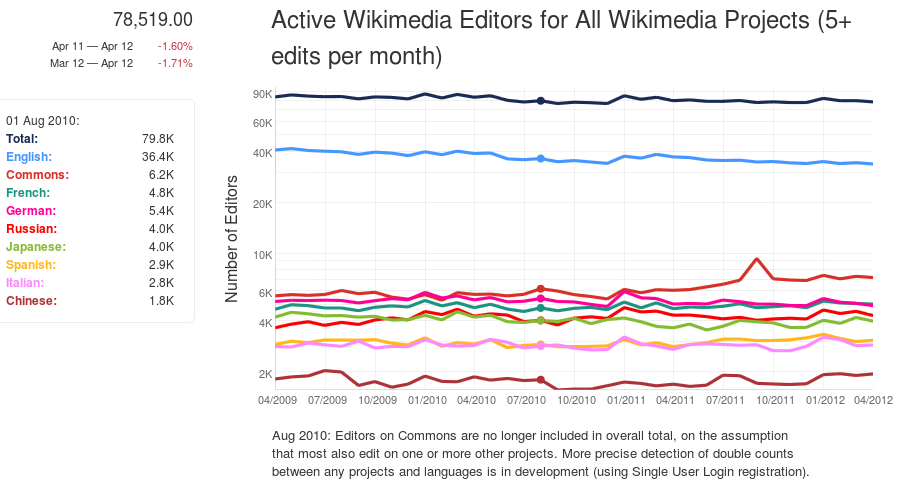
\includegraphics[width=\textwidth]{figs/wmflabs-reportcard}
  \caption{Example of the new reportcards produced by WMF.}
\end{figure}

\section{StatMediaWiki and Wikievidens}
StatMediaWiki~\footnote{\url{http://statmediawiki.forja.rediris.es/index_en.html}}
is another tool to calculate metrics and statistics about the evolution of any
MediaWiki-powered site, created by Emilio José Rodríguez (user \textit{Emijrp} in
Wikipedia). It also exports this pre-processed information for later consumption,
either as HTML pages or CSV data files. The code is licensed under GNU GPLv3.

\begin{figure}[h]
  \centering
    
\includegraphics[width=\textwidth]{figs/statMediaWiki}
  \caption{Project page for statMediaWiki at RedIRIS forge.}
\end{figure}

Wikievidens~\footnote{\url{http://code.google.com/p/wikievidens/}} can be 
seen as the evolution of the previous tool. It intends to provide a statistical
and visualization software for wikis. It is still on alpha stage.

\begin{figure}[h]
  \centering
    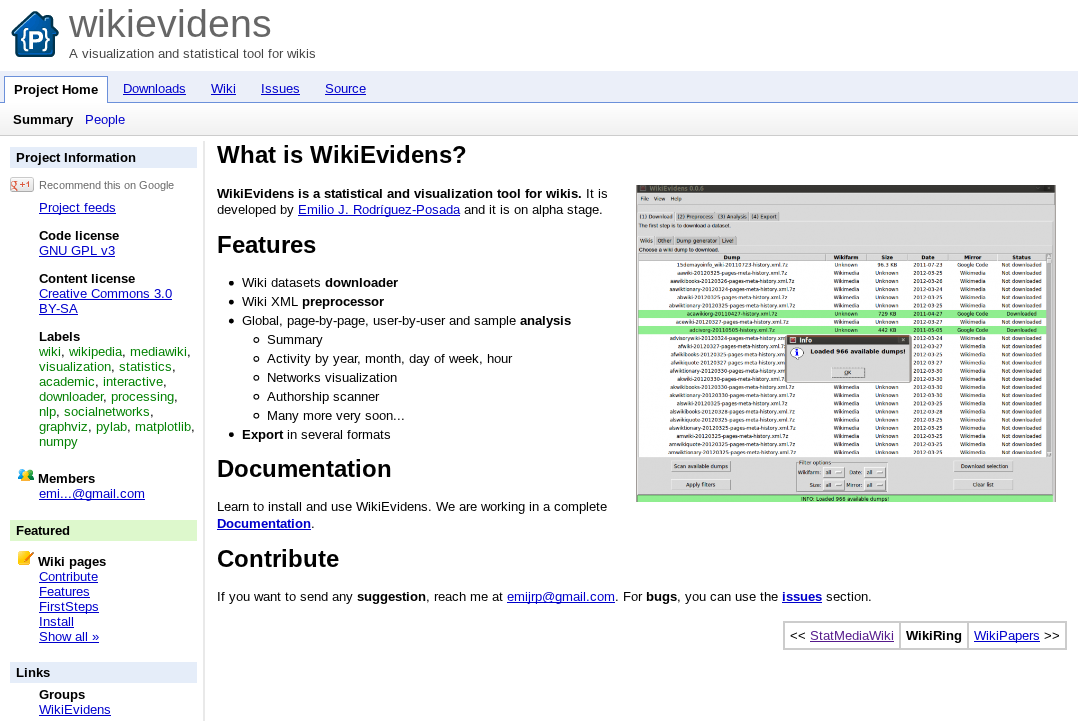
\includegraphics[width=\textwidth]{figs/wikievidens}
  \caption{Project page for wikievidens at Google Code.}
\end{figure}

\section{Interacting with the MediaWiki API}
Several libraries and applications have been developed to interact with the
MediaWiki API to automate certain tasks in Wikipedia, for instance developing bots
to peform regular maintentance duties. These tools can also be very useful for
researchers, since they provide convenient wrappers to access the API within
popular programming languages like Python.

\subsection{Pywikipediabot}
Pywikipediabot~\footnote{\url{http://www.mediawiki.org/wiki/Pywikipediabot}} is
a Python library created to facilitate the development of bots for Wikipedia.
As such, it is ideal to access MediaWiki API functionalities from Python. 
It is also very easy to learn, and there are
numerous examples that can be found illustrating existing bots to learn more
details about the library and how to write code with it.

However, you should take into account the usual recommendations for accessing
the Wikimedia API at a very fast pace, since you would run the risk of being banned
by system administrators or automated protection artifacts. Only bots that 
have been officially approved and get that status in the system can perform 
such actions at full speed.

\begin{figure}[h]
  \centering
    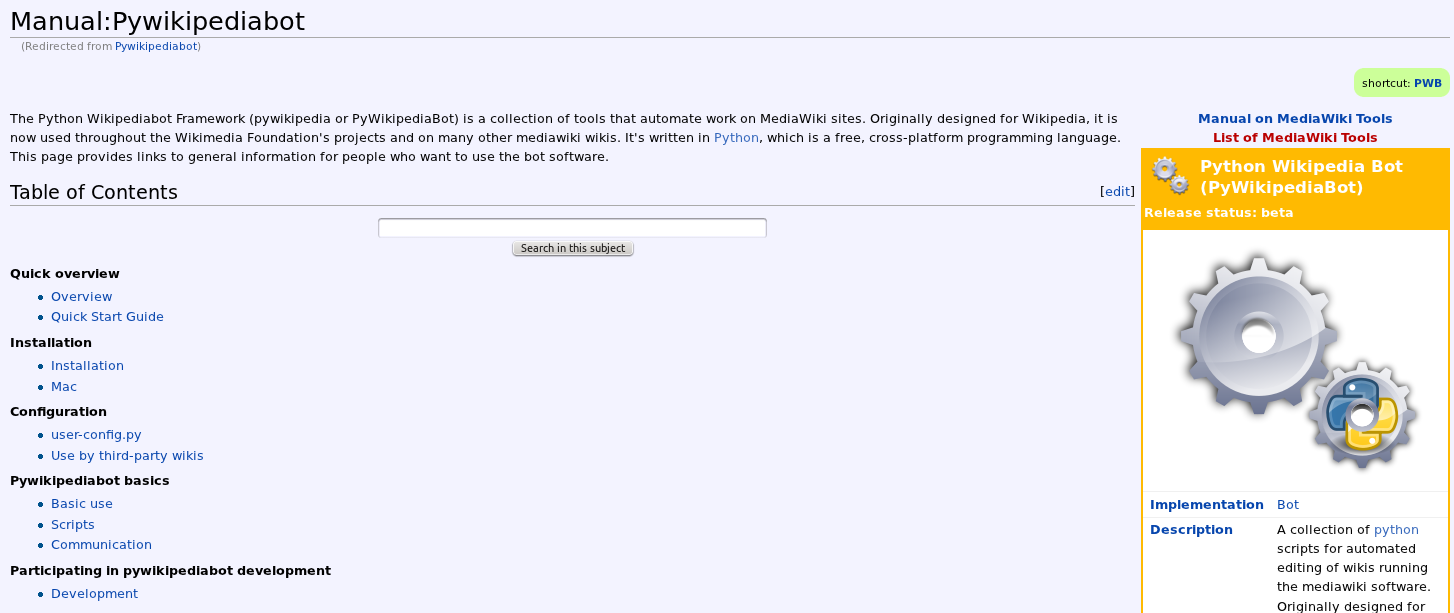
\includegraphics[width=\textwidth]{figs/pywikipediabot}
  \caption{Snapshot of the Pywikipediabot page at mediawiki.org}
\end{figure}

\subsection{Python-wikitools}
A second option for accessing the MediaWiki API from Python is 
python-wikitools~\footnote{\url{http://code.google.com/p/python-wikitools/}}. It
can be downloaded from the page project hosted at Google Code, or alternatively
through Pypy, the official Python packages repository.

\begin{figure}[h]
  \centering
    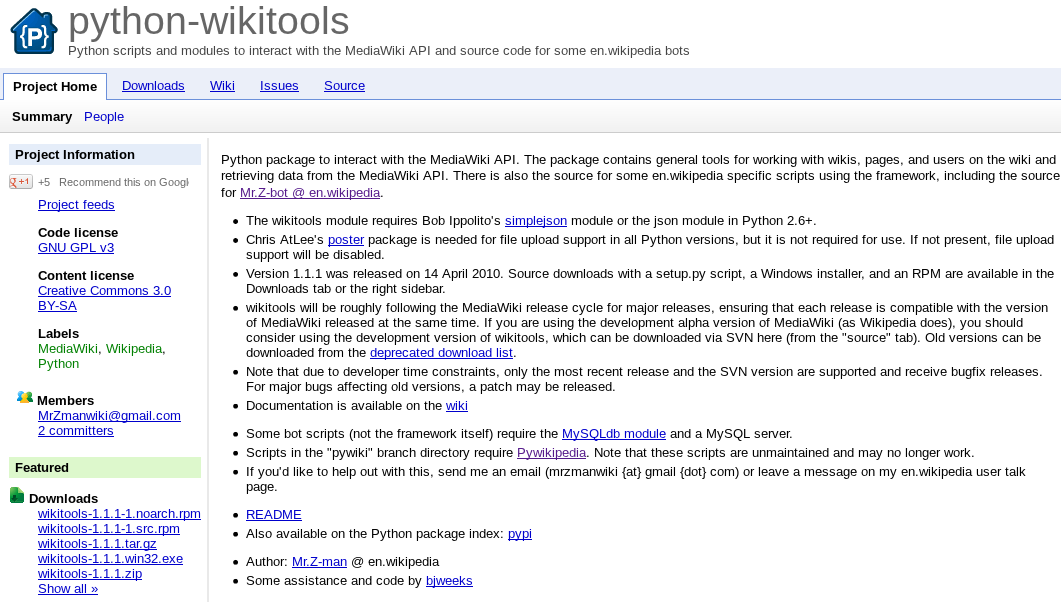
\includegraphics[width=\textwidth]{figs/python-wikitools}
  \caption{Snapshot of the python-wikitools at Google Code.}
\end{figure}

\subsection{Mwclient}
Finally, you can also check mwclient~\footnote{\url{http://sourceforge.net/projects/mwclient/}}, 
a framework for accessing
the MediaWiki API in Python written by Bryan Tong Minh for personal use in his own
bots. According to the information from the README file in the latest version
available (0.6.5):

\begin{quotation}
 \textit{Mwclient is a client to the MediaWiki API <\url{http://mediawiki.org/wiki/API}>
and allows access to almost all implemented API functions. Mwclient requires
Python 2.4. This version supports MediaWiki 1.11 and above. However, for 
functions not available in the current MediaWiki, a MediaWikiVersionError
is raised.}
\end{quotation}

\section{WikiTrust (for data analysis)}
WikiTrust~\footnote{\url{http://www.wikitrust.net/}} is an an open-source, 
on-line system to calculate reputation metrics for Wikipedia authors and content.
WikiTrust is hosted by the Institute for Scalable Scientific Data Management at 
the School of Engineering of the University of California, Santa Cruz, and their
main developers are Lucal de Alfaro, Bo Adler and Ian Pye. WikiTrust has been
one of the most popular research tools for calculating metrics about Wikipedia
authoring, including several research papers that can be accessed from the same
website. It has also been applied to the study of vandalism and reverted content
in Wikipedia, since along the process the software tracks the changes or moves
experimented by any word inside a Wikipedia article (as well as the author of
the revision performing those changes).

\begin{figure}[h]
  \centering
    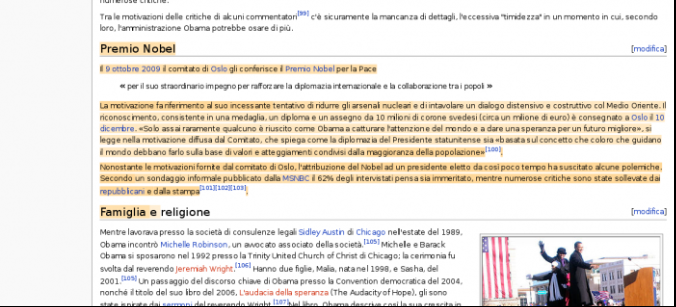
\includegraphics[width=\textwidth]{figs/wikitrust}
  \caption{Snapshot of the WikiTrust Firefox add-on in action, colouring Wikipedia
content according to the reputation metrics computed by the tool.}
\end{figure}

This authorship and reputation information is available online for being displayed
on any Wikipedia article thanks to an add-on plug-in developed for Mozilla 
Firefox~\footnote{\url{https://addons.mozilla.org/en-US/firefox/addon/wikitrust/}}.
A set of 3 different APIs~\footnote{\url{http://www.wikitrust.net/vandalism-api}} is
available for accessing the information computed by WikiTrust. The project authors
are actively lookin for support to provide these data for Wikipedia languages other
than English, after a power outage that brought down all international WikiTrust 
support once available.

The code is released under a BSD-like open source license. In addition, many
files implementing the core algorithm are written in Ocaml, a programming language
suitable for distributed processing in computer clusters. Since computing this algorithm
for an entire Wikipedia language is a daunting task, it must be accoplished by this
kind of parallel computing infrastructure. Even then, it can take a substantial
period of time to complete (nearly a month for the whole English Wikipedia, according
to the last comments from authors). This also depends on the number of nodes used
for the calculation.

\section{Pymwdat}
We can find traces of the first attemps to create applications to automate the 
analysis of Wikipedia data back to 2008. Dmitry Chichkov starts to develop wredese,
a tool to support the analysis of reverts and vandalism actions in Wikipedia. Later
on, this project became pymwdat~\footnote{\url{http://code.google.com/p/pymwdat/}},
a more general framework to implement these analyses, as well as the creation of
overall statistics about any Wikipedia language.

According to the online documentation for this project:

\begin{quotation}
\begin{verbatim}
 Requirements:
    * Python 2.6+, Linux;
    * OrderedDict (available in Python 2.7 or 
    http://pypi.python.org/pypi/ordereddict/)
    * 7-Zip (command line 7za)

Input Alternatives:
    * Wikipedia history dump 
    (e.g. enwiki-20100130-pages-meta-history.xml.7z);
    * Wikipedia page(s) name / category (use grab-pages.py);
    * Wikipedia page(s) history (.xml/.7z/.bz2/.gz).

Input Processing:
    * Detects reverts, reverted edits, revert wars, self-reverts;
    * Filtering, labeled revisions data sets management, etc;
    * Calculates users/page counters, revert rates, page diffs, etc 
    (~1 week/C2Duo/Full English Wikipedia dump).
\end{verbatim}

\end{quotation}


\section{Wikimedia-utilities}
Wikimedia-utilities~\footnote{\url{https://bitbucket.org/halfak/wikimedia-utilities}} 
is a very interesting piece of software that have not received general attention yet.
This software has been created by Aaron Halfaker, from Univ. of Minnesota, while
working in a Summer internship at Wikimedia Foundation premises in San Francisco.
The software is written in Python, and it has been conceived as a general-purpose
application that distributes the analysis of Wikipedia data dumps over different
subprocesses running on a multi-core machine.

The main advantage of this application is that it is extensible, namely that we can
extend the code to include additional calculations or any other tasks that we want
to peform on pages, revisions or their associated wiki text as the dump file
is decompressed. As an example, this baseline code has inspired the design of a 
new tool for tracking reverts of article content in Wikipedia accurately, written
by Fabian Flöck~\footnote{\url{http://people.aifb.kit.edu/ffl/reverts/}}.

\section{WikiDAT: Wikipedia Data Analysis Toolkit}
\label{sec:WikiDAT}
In April 2009, I released WikiXRay~\footnote{http://meta.wikimedia.org/wiki/WikiXRay},
a Python tool to automate the analyses included in my PhD. dissertation, comparing
the 10 largest Wikipedia languages at that time (by the official article count) from
different quantiative perspectives[[TODO:CITATION!!]]. The main advantage over other
similar tools is that WikiXRay also presents R code implementing the actual analysis
part, and not only the data extraction process (which was written in Python). So, this
is somehow one of the first available software for Wikipedia data analysis that really
made an effort to open up the data analysis part for other researchers to check the
code and reuse it for their own purposes.

However, advances in available libraries for XML parsing, and new proofs of concept
such as \textit{wikimedia-utilities} has made me thik that it could be a good idea
to try to rewrite the old code, creating an new tool that I have called WikiDAT
[[TODO:Citation]]. At the
time of writing, it is still in experimental phase as I am able to find free slots to
clean up and organize the multiple (and I have really many of them) code snippets that
I have created for undertaking past analyses with Wikipedia data.

At the time of writing (end of June, 2012) WikiDAT is shipped with new versions of
parsers for the \textit{pages-meta-history} and \textit{pages-logging} dump files.
Regarding the pages meta history, Tables[[TODO:internal-ref]] summarizes the data
fields that are currently extracted to a local MySQL database, organized in 5 different
tables:

\begin{itemize}
 \item Table \textit{page} stores information about all pages in a Wikipedia language.
 \item Table \textit{revision} contains metadata about all revisions performed in a
 Wikipedia language.
 \item Table \textit{revision\_hash} stores the id of every revision as well as
 an SHA-256 hash of the wiki text associated to it. 
 \item Table \textit{people} lists the numerical identifier and nickname of all
 registered users in a Wikipedia language.
 \item Table \textit{logging} with information about administrative and maintenance
 tasks undertaken in a Wikipedia language.
\end{itemize}

The original definition of these tables is based on the tables of the same name
defined in MediaWiki, except for table \textit{people} which is new. Fields in
bold characters identify keys to speed up search and sorting operations in database
queries.

\begin{longtable}[l]{|m{4.5cm}|m{5cm}|m{5cm}|}
 \caption[Table page in WikiDAT]
  {Fields and values included in table \textit{page} as defined in WikiDAT}
  \label{tab:table-page}\\
  \hline
  {\bfseries Field name} & {\bfseries Possible values} & {\bfseries Description}\\
  \hline
  {\bfseries page\_id} & Positive integer > 0 & Unique numerical id of the page \\
  \hline
  page\_namespace & Positive integer > 0  & Namespace of the page \\
  \hline
  page\_title & String, max. 255 characters & Title of the page \\
  \hline
  page\_restrictions & Binary string & Comma-separated set of permission keys 
  indicating who can move or edit this page (last revision)\\
  \hline
\end{longtable}

\begin{longtable}[l]{|m{4.5cm}|m{5cm}|m{5cm}|}
 \caption[Table people in WikiDAT]
  {Fields and values included in table \textit{people} as defined in WikiDAT}
  \label{tab:table-people}\\
  \hline
  {\bfseries Field name} & {\bfseries Possible values} & {\bfseries Description}\\
  \hline
  {\bfseries rev\_user} & Positive integer > 0 & Unique identifier of registered user \\
  \hline
  rev\_user\_text & String, max. 255 characters & Nickname of a registered user \\
  \hline
\end{longtable}

\begin{longtable}[l]{|m{4.5cm}|m{5cm}|m{5cm}|}
 \caption[Table revision in WikiDAT]
  {Fields and values included in table \textit{revision} as defined in WikiDAT}
  \label{tab:table-revision}\\
  \hline
  {\bfseries Field name} & {\bfseries Possible values} & {\bfseries Description}\\
  \hline
  {\bfseries rev\_id} & Positive integer > 0 & Unique identifier of a revision \\
  \hline
  rev\_page & Positive integer > 0 & Unique identifier of page modified in this 
  revision \\
  \hline
  rev\_user & Integer: -1, 0 or positive value & Unique identifier of registered user who performed
  this revision. -1 values indicate that user identifier was not recorded in the
  dump file; 0 values indicate anonymous users; positive values indicate identifier
  of registered users\\
  \hline
  rev\_timestamp & Date and time value (YYYY-MM-DD HH:MM:SS) & Timestamp for recording
  this revision in the database \\
  \hline
  rev\_len & Positive integer > 0  & Length in characters of the wiki page after this
  revision \\
  \hline
  rev\_parent\_id & Positive integer > 0 or NULL & Link to the numerical identifier of the
  previous revision undertaken in the same wiki page. NULL value indicates first revision for
  a wiki page \\
  \hline
  rev\_is\_redirect & Binary (1 or 0) & 1 value indicates that the page modified in this revision
  is a redirect \\
  \hline
  rev\_minor\_edit & Binary (1 or 0) & 1 value indicates that the user marked the \textit{minor
  edit} tick for this revision\\
  \hline
  rev\_fa & Binary (1 or 0) & 1 value indicates that, after this revision, the modified page
  displays the \textit{feature article} status tag (locale dependent). \\
  \hline
  rev\_comment & String (max. 255 characters) & Comment inserted by the user who
  performed this revision \\
  \hline
\end{longtable}

\begin{longtable}[l]{|m{4.5cm}|m{5cm}|m{5cm}|}
 \caption[Table logging in WikiDAT]
  {Fields and values included in table \textit{logging} as defined in WikiDAT}
  \label{tab:table-logging}\\
  \hline
  {\bfseries Field name} & {\bfseries Possible values} & {\bfseries Description}\\
  \hline
  {\bfseries log\_id} & Positive integer > 0 & Unique identifier of login actions \\
  \hline
  log\_type & String & Type of log action performed \\
  \hline
  log\_action & String & Concrete action undertaken (within a given type) \\
  \hline
  log\_timestamp & Date and time value (YYYY-MM-DD HH:MM:SS) & Timestamp for recording
  this log action in the database \\
  \hline
  log\_user & Positive integer > 0 & Unique identifier of registered user \\
  \hline
  log\_username & String & Nickname of user who carried out the log action \\
  \hline
  log\_namespace & Positive integer > 0 & Namespace of the page on which the log
  action was performed \\
  \hline
  log\_title & String (max. 255 characters) & Title of the page receiving the log
  action \\
  \hline
  log\_comment & String (max. 255 characters) & Comment of the log action \\
  \hline
  log\_params & String (max. 255 characters) & Additional descriptive params
  providing metadata about the log action (e.g. duration of a block) \\
  \hline
  log\_new\_flag & Positive integer > 0 & For Wikipedias with \textit{flagged-revisions} 
  enabled, rev\_id of the last flagged version of this page\\
  \hline
  log\_old\_flag & Positive integer > 0 & For Wikipedias with \textit{flagged-revisions} 
  enabled, rev\_id of the previous flagged version of this page\\
  \hline
\end{longtable}

The code of WikiDAT can be retrieved from the project site on Github[[TODO:link]].
The project files include some example implementations of common
analyses conducted on Wikipedia data, for descriptive purposes. The documentation
and source code in these examples will be improved progressively to provide
didactic case studies for other researchers interested in following similar approaches
in their own analyses. In the last chapter of this document we visit some of
these examples to illustrate some of these examle cases.

The following prerequisites must be satisfied to run the examples included in this
document, using the code included in WikiDAT:

\begin{itemize}
 \item MySQL server and client (v5.5 or later).
 \item Python programming language (v2.7 or later, but not the v3 branch) and 
 MySQLdb (v1.2.3).
 \item R programming language and environment (v 2.15.0 or later).
 \item Additional R libraries with extra data and functionalities:
 \begin{itemize}
  \item \textit{RMySQL}~\footnote{\url{http://cran.r-project.org/web/packages/RMySQL/index.html}}.
  \item \textit{lattice} (by Deepayan Sarkar).
  \item \textit{car} (by John Fox et al.).
  \item \textit{DAAG} (John Maindonald and W. John Braun) .
  \item \textit{Hmisc} (by Frank E Harrell Jr, with contributions from many other users).
  \item \textit{rjson} (by Alex Couture-Beil).
 \end{itemize}

\end{itemize}

Please, refer to Chapter~\ref{chap:methodology} introducing open source tools for data
analysis for additional information about obtaining and installing these dependencies.

%%%%%%%%%%%%%%%%%%%%%%%
%%%%%%%%%%%%%%%%%%%%%%%